%#####################################################################
%                           Chapter
%#####################################################################

%#####################################################################
\chapter{Implementation of Symmetric (Secret Key) Cryptography}
\thispagestyle{fancy}

\label{chap:symmetric_crypto}
%#####################################################################
The first part of this lecture deals with the (efficient) implementation of symmetric cryptographic algorithms, in particular \emph{block ciphers}. However, most of the concepts also apply to other primitives (hash functions, stream ciphers, \acp{MAC}) in a similar manner.

\section{Block Ciphers}
A block cipher is a function $bc\left(p,\,k\right)$ that maps (``encrypts'') a plaintext $p$ to a ciphertext $c$, given a key $k$. For given $k$, $bc$ is invertible (i.e., we can decrypt: $p = bc^{-1}\left(c,\,k\right)$). Both plaintext $p$ and ciphertext $c$ are of fixed \emph{block size} $n$ (measured in bit). The key is of fixed \emph{key size} $m$. A high-level block diagram for a typical block cipher is shown in Fig.~\ref{fig:symmetric_crypto:blockcipher}.

\begin{figure}[h!tb]
		\center
		\usetikzlibrary{shapes,arrows,calc}

\newcommand{\buswidth}[4][]{\draw (#2) node [#4=.6ex,#1] {#3} +(45:-.8ex) -- +(45:.8ex)}

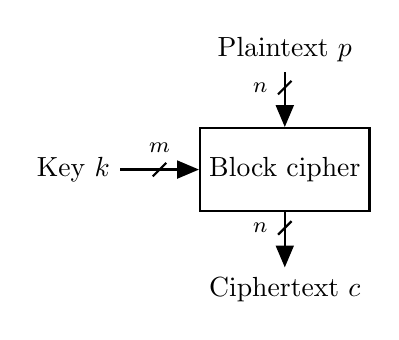
\begin{tikzpicture}
[
auto, thick, >=triangle 45,
block/.style    = {draw, thick, rectangle, minimum height = 3em, minimum width = 3em},
]
\node at (0,0)[block] (cipher) {Block cipher}; 
\draw[<-] (cipher.north) to ++(0,.7) node[above] {Plaintext $p$};
\draw[->] (cipher.south) to ++(0,-.7) node[below] {Ciphertext $c$};
\draw[<-] (cipher.west) to ++(-1,0) node[left] {Key $k$};

\buswidth{$ (cipher.north) + (0,.50)$}{\footnotesize $n$}{left}; 
\buswidth{$ (cipher.south) - (0,.20)$}{\footnotesize $n$}{left}; 
\buswidth{$ (cipher.west) - (0.5,0)$}{\footnotesize $m$}{above}; 
\end{tikzpicture} 
  	
		\caption{High-level view of a block cipher}
		\label{fig:symmetric_crypto:blockcipher}
\end{figure} 

\noindent A few examples for typical block ciphers with their respective key and block sizes are:

\begin{description}
	\item[\ac{AES}-128] The Rijndael~\cite{Daemen99} cipher with $n = m = 128$.
	\item[\ac{DES}] The \acl{DES}~\cite{fips_des} with $n = 64$, $m = 56$.
	\item[\ac{3DES}] Three \ac{DES} in \ac{EDE} configuration, $n = 64$, $m = 112$ or $m = 168$ (for 2-key and 3-key \ac{3DES}).
	\item[PRESENT] A lightweight block cipher~\cite{PresentCipher} with $n = 64$ and $m = 80$ or $m = 128$ (depending on selected key length).
\end{description}

Block ciphers are usually \emph{iterated} ciphers, i.e., a \emph{round function} is applied multiple times to map plaintext to ciphertext. Each round function operates on the \emph{state} of the cipher, that is usually initialized with the plaintext $p$ and hence of block size $n$. In a particular round $i$, a \emph{round key} $k_i$ (derived from the key $k$ using the \emph{key schedule}) enters the round function together with the current state $s_i$. The final state is then the ciphertext. Commonly, the round function of a block cipher follow one of two designs (although there are of course other approaches not covered here): the \emph{Feistel} design principle (\ac{DES}, \ac{3DES}, cf.~Fig.~\ref{fig:symmetric_crypto:feistel}) or the (newer) \ac{SPN} approach (\ac{AES}, PRESENT, cf.~Fig.~\ref{fig:symmetric_crypto:spn}). 

\begin{figure}[h!tb]
		\center
		\usetikzlibrary{shapes,arrows,calc}

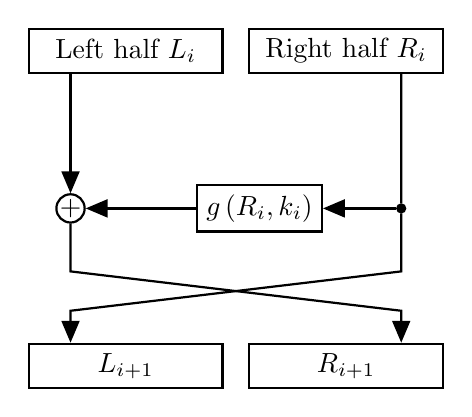
\begin{tikzpicture}
[
auto, thick, >=triangle 45,
block/.style    = {draw, thick, rectangle, minimum height = 1.6em, },
]
\node at (0,0)[block,minimum width = 7em] (left) {Left half $L_i$}; 
\node at (2.8,0)[block,minimum width = 7em] (right) {Right half $R_i$}; 

\node at (-.7,-2)[circle,draw,inner sep=0pt,minimum width=3mm] (xor) {+};
\node at (1.7,-2)[block] (f) {$g\left(R_i, k_i\right)$}; 

\node at (3.5,-2)[circle,draw,fill,inner sep=0pt,minimum width=1mm] (dot) {};

\node at (0,-4)[block,minimum width = 7em] (left2) {$L_{i+1}$}; 
\node at (2.8,-4)[block,minimum width = 7em] (right2) {$R_{i+1}$};

\draw[-] ($(right.south) + (0.7,0)$) -- ($(dot.north)$);
\draw[->] ($(dot.south)$) -- (3.5,-2.8) -- (-0.7,-3.3) -- ($(left2.north) - (0.7,0)$);
\draw[->] (dot) -- (f); 
\draw[->] (f) -- (xor);
\draw[->] ($(left.south) - (.7,0)$) -- (xor);
\draw[->] (xor) -- (-0.7,-2.8) -- (3.5,-3.3) -- ($(right2.north) + (0.7,0)$);
\end{tikzpicture} 
  	
		\caption{One round of a (balanced) Feistel cipher}
		\label{fig:symmetric_crypto:feistel}
\end{figure} 

\begin{figure}[h!tb]
		\center
		\usetikzlibrary{shapes,arrows,calc,decorations.markings}


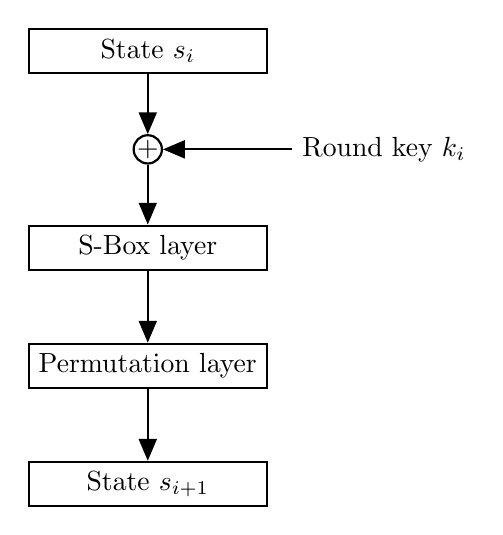
\begin{tikzpicture}
[
auto, thick, >=triangle 45,
block/.style    = {draw, thick, rectangle, minimum height = 1.6em, },
]
\node at (0,0)[block,minimum width = 8.6em] (state) {State $s_i$}; 
\node at (0,-1.25)[circle,draw,inner sep=0pt,minimum width=3mm] (xor) {+};
\node at (3,-1.25)[] (k) {Round key $k_i$};
\node at (0,-2.5)[block,minimum width = 8.6em] (sbox) {S-Box layer}; 
\node at (0,-4)[block,minimum width = 8.6em] (p) {Permutation layer}; 
\node at (0,-5.5)[block,minimum width = 8.6em] (state2) {State $s_{i+1}$}; 

 \draw[->] (state) -- (xor); 
 \draw[->] (xor) -- (sbox); 
 \draw[->] (sbox) -- (p); 
 \draw[->] (p) -- (state2); 
  \draw[->] (k) -- (xor); 
  
\end{tikzpicture} 
   	
		\caption{One round of an \ac{SPN} cipher (note that the key addition may also happen at the end of the round)}
		\label{fig:symmetric_crypto:spn}
\end{figure} 

\subsection{Building Blocks}
To provide cryptographic security, block ciphers require elements to provide ``diffusion'' (``a single input bit change affects all output bits with 50\% probability'') and ``confusion'' (``the relationship between input and output is sufficiently complex''). The core elements to reach these goals in virtually all block ciphers are:

\begin{description}
  \item[Key addition] The key is combined with the plaintext / the state through an addition-like operation, normally bitwise \ac{XOR} or arithmetic addition over a finite ring (e.g., $\mod 2^{32}$).
	\item[\acs{SBOX}] A \ac{SBOX} is a non-linear mapping, usually over a small number of bits (e.g. 8-to-8 or 6-to-4). A cipher may have multiple, different \acp{SBOX} (like the \ac{DES}) or one one single \ac{SBOX} (e.g., \ac{AES} or PRESENT). The \ac{SBOX} may be (seemingly) chosen at random (\ac{DES}, PRESENT) or follow an algebraic structure (\ac{AES}). Provides ``confusion''.
	\item[Permutations] A linear mapping to provide ``diffusion'', permuting the output of the \ac{SBOX} layer such that one \ac{SBOX} output bit affects multiple \ac{SBOX} inputs in the next round. Can be realized bitwise (like in \ac{DES}, PRESENT) or through bytewise/wordwise operations (like in the \ac{AES}). 
\end{description}

To give an example, the PRESENT block cipher ($n$ = 64, $m$ = 80) is given in the following pseudocode:

\begin{algorithm}
\center
\begin{algorithmic}
\vspace{2mm}
\State $s \gets p$ 
\State $k_i \gets$ \Call{generateRoundKeys}{$k$}


\For{i = 1 ... 31}
	\State $s \gets$ \Call{addRoundKey}{$s$, $k_i$}
	\State $s \gets$ \Call{sboxLayer}{$s$}
	\State $s \gets$ \Call{pLayer}{$s$}
\EndFor

\State $c \gets$ \Call{addRoundKey}{$s$, $k_{32}$}

\vspace{2mm}
\end{algorithmic}
\caption{PRESENT (pseudocode based on~\cite{PresentCipher})}
\label{alg:symmetric_crypto:present}
\end{algorithm}

The \verb+addRoundKey+ operation is simple bitwise \ac{XOR} of the state $s$ and the round key $k_i$. The \verb+sboxLayer+ operation applies the 4-to-4 PRESENT \ac{SBOX} to the state in groups of 4 bit each, i.e., the \acs{SBOX} is applied a total of $\nicefrac{64}{4} = 16$ times. The PRESENT \ac{SBOX} is given in the following Table~\ref{tab:symmetric_crypto:present} (as hexadecimal digits):

\begin{table}[htbp]
	\centering
		\begin{tabular}{c | c c c c c c c c c c c c c c c c}
			$x$    & 0 & 1 & 2 & 3 & 4 & 5 & 6 & 7 & 8 & 9 & A & B & C & D & E & F \\\hline
      $S(x)$ & C & 5 & 6 & B & 9 & 0 & A & D & 3 & E & F & 8 & 4 & 7 & 1 & 2
		\end{tabular}
	\caption{PRESENT \ac{SBOX}}
	\label{tab:symmetric_crypto:present}
\end{table}

% // bit i goes to position i/4 + (i mod 4) * 16
The \verb+pLayer+ operation is a bitwise permutation, whereas the bit at position $j$ is permuted to position

$$
j_p = \left\lfloor \frac{j}{4} \right\rfloor + \left( j\ \textrm{mod}\ 4 \right) \times 16
$$

i.e., bit~0 is permuted to position 0, bit~1 to 16, bit~2 to 32, bit~3 to 48, bit~4 to 1, and so on. The original paper~\cite{PresentCipher} supplies this as a full table. We will discuss the cost of each of these core operations (in software and hardware) in the following, using the example of PRESENT again.

\paragraph{A Note on Bitwise Operations in \texttt{C}}
To implement bitwise permutations (and other bitwise manipulations), usually two primitive operations are required: getting the value of a bit in a word (\texttt{getbit}) and setting/clearing a bit in a word (\texttt{setbit} and \texttt{clrbit}). In \texttt{C}, assuming the variable \texttt{word} is a byte (type \texttt{uint8\_t}), this can be implemented as follows:

\begin{verbatim}
uint8_t getbit(const uint8_t word, const uint8_t bit)
{
    return (word >> bit) & 0x1;
    // or, if return value != 0 means: bit set
    // return (word & (1 << bit));
}

void setbit(const uint8_t* word, const uint8_t bit)
{
    *word |= (1 << bit);
}

void clrbit(const uint8_t* word, const uint8_t bit)
{
    *word &= ~(1 << bit);
}

\end{verbatim}
 
Note that this is the most straightforward approach and can be often optimized. Also, note that using dedicated functions for this task can cause significant runtime overhead, therefore, usually macros are used for these operations. 
%
On some platforms, there are dedicated assembly instructions for manipulating bits in a register, e.g., \texttt{SBR} and \texttt{CBR} to set and clear bits in a register in the Atmel AVR architecture\footnote{\url{http://www.atmel.com/webdoc/avrassembler/avrassembler.wb_SBR.html} and \url{http://www.atmel.com/webdoc/avrassembler/avrassembler.wb_CBR.html}}, as well as the equivalent for the MSP430 with \texttt{BIS} and \texttt{BIC}\footnote{\url{https://www.ti.com/sc/docs/products/micro/msp430/userguid/as_5.pdf}} or the ARM Cortex M0 with \texttt{ANDS}, \texttt{ORS}, \texttt{BICS}\footnote{\url{http://infocenter.arm.com/help/index.jsp?topic=/com.arm.doc.dui0497a/CIHJJEIH.html}}. 

These specific instructions usually avoid the load, update, store cycle required when directly translating the above \texttt{C} code. Note that optimizing compilers for these architectures often recognize the above constructs and automatically replace them with the appropriate assembly instruction.


\subsection{Key Addition Layer}
Since the key addition is, as mentioned, usually \ac{XOR} or rarely arithmetic addition, it is cheap both in hardware (\ac{XOR} gates are a basic building block) and software (nearly every processor has dedicated \verb+XOR+ and \verb+ADD+ instructions). Due to the simplicity of the operation, there is usually no or very little optimization potential (i.e., by unrolling the loop that performs the \ac{XOR}) at all. 


\subsection{\acs{SBOX} Layer}
\label{chap:symmetric_crypto:sbox}
In software implementations, the \ac{SBOX} is normally realized as a \ac{LUT} (i.e., an array stored in \ac{RAM} or Flash) and hence normally fast. However, the following optimizations (and probably more) may be considered:

\begin{itemize}
	\item Ciphers with multiple, different \acp{SBOX} (e.g., \ac{DES}) have higher memory requirements and are hence less suited for compact software implementations.
	
	\item To optimize for execution time, it may be beneficial to merge multiple \ac{SBOX} instances into one look-up, e.g., for PRESENT, two 4-to-4 lookups can be done in parallel by using an 8-to-8 \ac{LUT}.
	
	\item Depending on the hardware platform, certain memories can be faster. For example, a read from \ac{RAM} may take one cycle, while a Flash access needs two cycles. Hence, it could be beneficial to load the \ac{SBOX} into \ac{RAM} (if sufficient space is available) before carrying out encryption.	
	
	\item If memory complexity is to be minimized, a smaller \ac{SBOX} is generally better. For example, to store a $a$-to-$b$ bit \ac{SBOX}, $b \times 2^a$ bit storage are needed at least---for example, for PRESENT, the 4-to-4 \ac{SBOX} needs at least 64~bit = 8~byte to be stored. Note that, however, most architectures do not allow addressing below the byte level, so additional (time) overhead will be incurred to correctly apply the \ac{SBOX}. Commonly, \acp{SBOX} are not larger than 8-to-8 (as in \ac{AES}), which already requires 256~byte for storage.
\end{itemize}

To further illustrate the last point, consider the 4-to-4 PRESENT \ac{SBOX}. In \verb+C+ syntax, this \ac{SBOX} would be stored in an array, and a look-up performed on a single state byte \verb+s+ as in the following example:

\lstset{language=C}
\begin{lstlisting}
const uint8_t sbox[16] = { 0xC, 0x5, 0x6, 0xB, 0x9, 0x0, 0xA, 0xD, 
    0x3, 0xE, 0xF, 0x8, 0x4, 0x7, 0x1, 0x2 };

// Look-up lower nibble
uint8_t s_new = sbox[s & 0x0F];

// Look-up upper nibble
s_new |= sbox[(s >> 4) & 0x0F] << 4;

// Update state
s = s_new;
\end{lstlisting}

However, the additional bit shifts and boolean operations create significant overhead. Hence, the idea is to merge two instances of the \ac{SBOX} by using a larger, 256-byte table of the following structure ($sb\left(in\right)$ is the 4-bit output value, $|$ indicates concatenation of two nibbles to a full byte):
$$
\left(\begin{array}[h!tbp]{c c c c c}
	sb\left(0x0\right)\,|\,sb\left(0x0\right) & sb\left(0x0\right)\,|\,sb\left(0x1\right) & sb\left(0x0\right)\,|\,sb\left(0x2\right) & \ldots & sb\left(0x0\right)\,|\,sb\left(0xF\right) \\
	sb\left(0x1\right)\,|\,sb\left(0x0\right) & sb\left(0x1\right)\,|\,sb\left(0x1\right) & sb\left(0x1\right)\,|\,sb\left(0x2\right) & \ldots & sb\left(0x1\right)\,|\,sb\left(0xF\right) \\
	sb\left(0x2\right)\,|\,sb\left(0x0\right) & sb\left(0x2\right)\,|\,sb\left(0x1\right) & sb\left(0x2\right)\,|\,sb\left(0x2\right) & \ldots & sb\left(0x2\right)\,|\,sb\left(0xF\right) \\
	\multicolumn{5}{c}{\ldots} \\
	sb\left(0xF\right)\,|\,sb\left(0x0\right) & sb\left(0xF\right)\,|\,sb\left(0x1\right) & sb\left(0xF\right)\,|\,sb\left(0x2\right) & \ldots & sb\left(0xF\right)\,|\,sb\left(0xF\right) \\
\end{array}\right)
$$

In (abbreviated) \verb+C+, this translates to:

\lstset{language=C}
\begin{lstlisting}
const uint8_t sbox[256] = { 
	0xCC, 0xC5, 0xC6, ..., 0xC1, 0xC2, // up: sb(0x0) = 0xC 
	0x5C, 0x55, 0x56, ..., 0x51, 0x52, // up: sb(0x1) = 0x5
	...
	0x1C, 0x15, 0x16, ..., 0x11, 0x12, // up: sb(0xE) = 0x1
	0x2C, 0x25, 0x26, ..., 0x21, 0x22, // up: sb(0xF) = 0x2
};

// Look-up two nibbles in parallel
s = sbox[s]
\end{lstlisting}

In hardware, there are two basic ways to realize an \ac{SBOX}: as a \ac{LUT} (using \ac{RAM} or other memories) or in combinatorial logic. In the latter case, each output bit is represented as a Boolean expression in the input bits. These functions are then implemented using logic gates (e.g., \verb+AND+, \verb+NAND+, \verb+OR+, \verb+NOR+, \verb+XOR+).  
While we do not focus on hardware implementations in this lecture, this concept is explained here since it has relevance for certain software optimizations as well.

Taking a 4-to-4 \ac{SBOX} as an example, this results in four Boolean expressions:

\begin{align}
	r_0 &= sb_0 \left(in_0, in_1, in_2, in_3 \right) \nonumber \\
	r_1 &= sb_1 \left(in_0, in_1, in_2, in_3 \right) \nonumber \\
	r_2 &= sb_2 \left(in_0, in_1, in_2, in_3 \right) \nonumber \\
	r_3 &= sb_3 \left(in_0, in_1, in_2, in_3 \right) \nonumber
\end{align}

where $in = in_3 in_2 in_1 in_0$ is the binary representation of the \ac{SBOX} input and $r = r_3 r_2 r_1 r_0$ the one of the output. The Boolean expressions $sb_i$ can be written using standard techniques, e.g., in \ac{CNF}~\cite{wiki:cnf}, \ac{DNF}~\cite{wiki:dnf}, and \ac{ANF}~\cite{wiki:anf}. Karnaugh maps~\cite{wiki:karnaugh} can be used to minimize the circuit complexity.

A simple example for such a Boolean function (unrelated to any real \ac{SBOX}) in \ac{DNF} would be:
$$
sb_0 \left(in_0, in_1, in_2, in_3 \right) = \left(in_0 \wedge \overline{in_1} \wedge in_3\right) \vee \left(in_1 \wedge in_2\right) \vee \left(\overline{in_3}\right)
$$

Note that it would be also possible to use Boolean expressions in software implementations (computing every output bit separately), however, the overhead both in code size and execution time would be prohibitive in virtually all practical scenarios. Yet, as mentioned, certain software optimizations (see Sect.~\ref{sec:symmetric_crypto:bitslicing}) are still based on this approach.

\subsection{Permutation Layer}
The efficiency of permutations in software highly depends on the type of permutation: permutations on the byte (or multiple-of-byte) level are generally fast since the addressing scheme of processors usually allows to copy a single byte. For example, the \ac{AES} was designed with fast software implementations in mind, hence, the permutation layer (\verb+ShiftRows+ and \verb+MixColumns+) operates on a byte or word level. A \verb+C+ example for such a byte-wise permutation would be:

\lstset{language=C}
\begin{lstlisting}
// Permute bytes 0, 1, 2, 3 -> 2, 3, 1, 0
const uint8_t tmp = s[0];
s[0] = s[2];
s[2] = s[1];
s[1] = s[3];
s[3] = tmp;

\end{lstlisting}

In contrast, bit-wise permutations are less efficient to implement, as every bit has to be extracted and copied to its output position. For example, moving the single bit~14 (byte position~$\left\lfloor \nicefrac{14}{8} \right\rfloor = 1$, bit position~$\left(14\ \textrm{mod}\ 8\right) = 6$) to bit~36 (byte~4, bit~4) would be implemented as:

\lstset{language=C}
\begin{lstlisting}
// Byte 1, bit 6 to byte 4, bit 4
// Get source bit
const uint8_t tmp = (s[1] >> 6) & 0x1; 
// Assume out is zeroed before
out[4] |= tmp << 4;
\end{lstlisting}

Note that such operations have to be carried out for each bit (e.g., 64~times in the case of PRESENT or 32~times for \ac{DES}) and are harder to realize \emph{in-place} (e.g., a separate output buffer is needed).

In contrast, in hardware implementations, permutations are usually ``free'' since they represent simple interconnects. \ac{DES}, for example, was designed as a cipher fast in hardware and hence makes extensive use of bitwise permutations. \ac{AES} was designed for software and implementation on 8-bit (or higher) processors. PRESENT represents a ``middle ground'' for a very lightweight cipher that is fast or small both in hardware and software (even on extremely constrained 4-bit \acp{muC}).

\section{Table-based Software Optimizations}
As pointed out in the previous section, bitwise permutations are in general expensive in software. In this section, we discuss one approach to mitigate this problem. Section~\ref{sec:symmetric_crypto:bitslicing} then discusses an alternative approach that may give further speed-up in certain scenarios. As we have already seen in Section~\ref{chap:symmetric_crypto:sbox}, spending slightly more memory may speed up operations considerably. 

The core idea of this section is twofold: On the one hand, we merge the \ac{SBOX} and permutation layer into one operation. Secondly, we generate tables with output size that is as big as the internal state, i.e., while a normal PRESENT \ac{SBOX} is 4-to-4~bit, we now use a 4-to-64~bit table. Again, recall that storing and $a$-to-$b$~bit table requires $b \times 2^a$~bit, i.e., increasing the output size $b$ only linearly affects the overall table size (not exponential like $a$). Hence, the memory overhead stays within reasonable limits (e.g., $64 \times 2^4 = 1024$\,bit instead of $4 \times 2^4 = 64$\,bit).

Before looking at a ``real'' example for the approach of this section, consider an artificial byte-oriented cipher with a 4-byte (32-bit) state. Assume that the same \ac{SBOX} is applied to each state byte, followed by the byte permutation $\left(0, 1, 2, 3\right) \rightarrow \left(2, 3, 1, 0\right)$.
A straightforward implementation would be:

\lstset{language=C}
\begin{lstlisting}
// Apply S-Box
for(uint8_t i = 0; i < 4, i++)
{
   s[i] = sbox[s[i]];
}

// Permute bytes 0, 1, 2, 3 -> 2, 3, 1, 0
const uint8_t tmp = s[0];
s[0] = s[2];
s[2] = s[1];
s[1] = s[3];
s[3] = tmp;

\end{lstlisting}

However, note that the \ac{SBOX} and permutation layer can be easily merged in this case, saving four write operations to the state:

\lstset{language=C}
\begin{lstlisting}
// Permute bytes 0, 1, 2, 3 -> 2, 3, 1, 0 and apply S-Box
const uint8_t tmp = s[0];
s[0] = sbox[s[2]];
s[2] = sbox[s[1]];
s[1] = sbox[s[3]];
s[3] = sbox[tmp];
\end{lstlisting}

For ciphers with byte-oriented permutations (like \verb+ShiftRows+ in the \ac{AES}), this optimization has a relatively minor effect, since the permutation layer is in any case computationally efficient. On the other hand, for bitwise permutations, the above method cannot be applied directly since multiple bytes are affected by each \ac{SBOX} output. This is where ``artificially'' increasing the table output length to the full state size comes into play: the output bits of the \ac{SBOX} are directly stored at their \emph{permuted} output positions, while the remaining state bits are set to zero. 

To illustrate this concept, consider the PRESENT \ac{SBOX} for the first state byte $s_0$. In binary, the \ac{SBOX} is given as:
\begin{align}
	0xC &= \left(1100\right)_2 \nonumber \\ 
	0x5 &= \left(0101\right)_2 \nonumber \\ 
	0x6 &= \left(0110\right)_2 \nonumber \\
	\ldots \nonumber \\
	0x2 &= \left(0010\right)_2 \nonumber 
\end{align}
 

The four output bits after the permutation affected by this \ac{SBOX} output are bit~0, bit~16, bit~32, and bit~48. In the new table, we store the full width of the state, with the output bits moved to the correct positions:  
\begin{align}
	& \left( 0 \ldots 0\underline{1}0 \ldots 0\underline{1}0 \ldots 0\underline{0}0 \ldots 00\underline{0}\right)_2 \nonumber \\ 
	& \left( 0 \ldots 0\underline{0}0 \ldots 0\underline{1}0 \ldots 0\underline{0}0 \ldots 00\underline{1}\right)_2 \nonumber \\ 
	& \left( 0 \ldots 0\underline{0}0 \ldots 0\underline{1}0 \ldots 0\underline{1}0 \ldots 00\underline{0}\right)_2 \nonumber \\ 
	& \ldots \nonumber \\
	& \left( 0 \ldots 0\underline{0}0 \ldots 0\underline{0}0 \ldots 0\underline{1}0 \ldots 00\underline{0}\right)_2 \nonumber \\ 
\end{align}

This means that in the output of the table for the first \ac{SBOX}, only the bits~0, 16, 32, and 48 can ever take a non-zero value. For the second \ac{SBOX}, there is a \emph{separate}, different table with only the bits~1, 17, 33, and 49 changing, i.e., we have the pattern:
$$
\left( 0 \ldots \underline{x}00 \ldots \underline{x}00 \ldots \underline{x}00 \ldots 0\underline{x}0\right)_2
$$
In total, this yields 16 4-to-64 tables, one for each \ac{SBOX}. Note that now the table for every \ac{SBOX} instance is different due to the different permuted positions. The final question is how to re-combine the outputs of each table into one state. This can be easily achieved using bitwise \verb+XOR+ or \verb+OR+ operations, which both yield the desired result because there is never more than one non-zero bit per bit position\footnote{As a side question, think about why bitwise \texttt{AND} would \emph{not} be suitable.}. 

The following \verb+C+ code illustrates the implementation of this technique for two \acp{SBOX}:

\begin{lstlisting}
const uint64_t spbox0[16] = { 
    0x0001000100000000ULL, 0x0000000100000001ULL, 
    0x0000000100010000ULL, ..., 0x0000000000010000ULL };
const uint64_t spbox1[16] = { ... };
...
// Look-up lower nibble
uint64_t s_new = spbox0[s & 0x0F];
// Look-up upper nibble and XOR into state
s_new ^= spbox1[(s >> 4) & 0x0F];
...

\end{lstlisting}

\paragraph{Why does this work?} 
The key reason is that it is by definition impossible that we have two non-zero bits at the \emph{same position} when combining (\verb+XOR+ing) multiple ``S-P-Box'' outputs. That is, at every bit position, there is at most one 1 and (in the case of PRESENT) fifteen 0 bits. \verb+XOR+ (and also \verb+OR+) has the property that $1 \oplus 0 = 1$ but $0 \oplus 0 = 0$. Obviously, without the guarantee that there is at most one 1 per bit position, the optimization would \emph{not} work.

\paragraph{Efficiency and Cost}
By combining the \ac{SBOX} and permutation layer into slightly bigger, individual tables, we gain significant speed-up as bit permutations are completely avoided. The disadvantage lies in the memory requirements. While a straightforward PRESENT \acp{SBOX} consumes $4 \times 2^4 = 64\,\textrm{bit} = 8\,\textrm{byte}$, the combined tables require $16 \times 64 \times 2^4 = 16384\,\textrm{bit} = 2048\,\textrm{byte}$ of storage (the additional factor 16 is due to the fact that we now have one table per \ac{SBOX}, rather than one shared \ac{LUT}). This is a significant overhead, however, of course some amount of program code memory (for implementing the permutation) is saved. 

If the size of the table is of concern, note that due to the regular structure of the PRESENT permutation, it would be possible to save memory by storing the combined table once, looking-up a value, and shifting it left by one for each \ac{SBOX} (i.e. no shift if first \ac{SBOX}, shift by one for second \ac{SBOX}, and so on). This single table would then be $64 \times 2^4 = 1024\,\textrm{bit} = 128\,\textrm{byte}$ long.

In addition, for PRESENT, further speed improvements could be reached by combining the table-based approach with the ``merge two \acp{SBOX}'' idea explained in Section~\ref{chap:symmetric_crypto:sbox}. To store these tables, $8 \times 64 \times 2^8 = 131072\,\textrm{bit} = 16384\,\textrm{byte} = 16\,\textrm{kByte}$ would be needed, but the runtime for the combined \ac{SBOX} look-up and permutation would be approximately halved overall. Again, using the above ``shifting'' approach, the size could be brought down by a factor of 8 to $64 \times 2^8 = 16384\,\textrm{bit} = 2048\,\textrm{byte}$.

For the \ac{AES}, there is a variant of these table-based optimizations called \emph{T tables}, exploting some properties of the \verb+MixColumns+ transform for very fast implementation on 32-bit platforms. This optimization is further explained in the original \ac{AES} proposal~\cite[Section 5.2]{Daemen99}.


\section{Bitslicing}
\label{sec:symmetric_crypto:bitslicing}
Rather than ``working around'' the problem of efficiently performing bitwise permutations by using tables, the \emph{bitslicing} method explained in this section takes a radically different approach to the problem of fast implementation of symmetric cryptography in software. First introduced by Biham in~\cite{Biham1997}, it makes use of the fact that often, one has to encrypt many block of plaintext at the same time (e.g., for disk encryption, network transfers, exhaustive key search, to name a few). 

The core idea is best explained by revisiting the problem of permutations again---they are fast as long as they are done on the level of the smallest addressable unit on a processor, i.e., normally a byte. In theory, one could realize a bitwise permutation (with significant storage overhead) by storing each bit of the state in a individual byte (leaving the remaining 7~bit set to zero), and then permuting the respective bytes. However, that would mean that one would need---for the example of a cipher with 64-bit state---64~byte, of which only $\nicefrac{1}{8}$ are used. Bitslicing allows to ``reclaim'' the bits that would be ``wasted'' in the above approach. 

However, let us for now follow the approach of storing one bit per byte in order to see how an implementation of the typical components of a block cipher would look like. We assume that both plaintext and the key (round keys) are stored in this form. In \verb+C+, we would the have an structure as in the following example:

\begin{lstlisting}

// Plaintext = 0xF9 ... AC = 11111001 ... 10101100
uint8_t state[64] = {0, 0, 1, 1, 0, 1, 0, 1, ..., 
   1, 0, 0, 1, 1, 1, 1, 1 };

uint8_t key[64] = {0, 1, 1, 0, ...};	

for(uint8_t round = 1; round <= 31; round++)
{
   // Key addition
   // S-Box
   // Permutation
   // Round key update
}
\end{lstlisting}

\paragraph{Key Addition Layer}
Since both round key and state are in the ``expanded'' form, we can simply XOR them byte-wise, whereas each XOR between two bytes of course only takes care of one bit in the state. The \verb+C+ pseudocode would be:

\begin{lstlisting}
for(uint8_t i = 0; i < 64; i++)
{
   state[i] = state[i] ^ roundkey_exp[i];
}
\end{lstlisting}

\paragraph{Permutation Layer}
The bitwise permutation of PRESENT now becomes a byte-wise permutation (due to the wasteful way of storing the state bits). For example, for the first few bits of the PRESENT permutation, this would result in (assuming the permutation is not done in-place):
\lstset{language=C}
\begin{lstlisting}
state_out[0]  = state[0];
state_out[16] = state[1];
state_out[32] = state[2];
state_out[48] = state[3];
state_out[1]  = state[4];
// ...
\end{lstlisting}

\paragraph{\ac{SBOX} Layer}
In the new, bit-wise representation, the \ac{SBOX} can no longer easily implemented as a \ac{LUT}\footnote{While one could of course still ``collect'' input bits, look-up the output in a \ac{LUT}, and map the output bits back onto bytes, this would be quite inefficient.}. Instead, we represent the \ac{SBOX} output bits as Boolean functions in the input bits as explained in Section~\ref{chap:symmetric_crypto:sbox}. In the following, we will mainly use the \acl{ANF} representation (for details, cf.~Section~\ref{chap:symmetric_crypto:anf}). For example, the \ac{ANF} of the first output bit $y_0 \in \binfield{}$ of the PRESENT \ac{SBOX} (with input $\left(x_0,\,x_1,\,x_2,\,x_3\right) \in \binfield{4})$ is given as:
$$
y_0 = x_0 + x_1 \cdot x_2 + x_2 + x_3
$$

Hence, we can (again not in-place) implement the \ac{SBOX} layer as follows:
\lstset{language=C}
\begin{lstlisting}
// First S-Box, first bit
state_out[0]  = state[0] ^ (state[1] & state[2]) ^ state[2] ^ state[3];
...
// Second S-Box, first bit
state_out[4]  = state[4] ^ (state[5] & state[6]) ^ state[6] ^ state[7];
...
\end{lstlisting}

By writing the expression of the other \ac{SBOX} output bits, we can hence implement the \ac{SBOX} using Boolean operations only.
The most important observation to understand the working principle of bitslicing is the following:

\begin{quote}
All operations that we use (permuting bytes, applying Boolean operators) work \emph{bitwise}, i.e., they operate on each bit independently. Hence, we can reclaim the ``remaining'' bits (so far set to zero) in each byte by storing a second block of plaintext in the second bit, in the third bit, and so on. We effectively execute the cipher \emph{eight times in parallel}!
\end{quote}

There are no further modifications needed to the above implementations of the blocks, the only requirement is to store the plaintext blocks $p_i$ (each for example each with size 8~byte) in the correct way into the bitsliced state $s'\left[0 ... 63\right]$ (with for example 64~bytes for 64~state bits): the first (least significant) bit of the first block $p_0$ goes into bit~0 of $s'\left[0\right]$, the second bit of $p_0$ into bit~0 of $s'\left[1\right]$, and so on. The first bit of the second block $p_1$ goes into bit~1 of $s'\left[0\right]$, the second bit of $p_1$ into bit~1 of $s'\left[1\right]$, and so on, until all 8~block are stored in $s'$. After the above operations (key addition, \ac{SBOX}, permutation) have been carried out and the cipher is completely executed, one has to map back $s'$ to a normal representation. The two representations (normal and bitsliced form) are illustrated in Figure~\ref{fig:symmetric_crypto:bitslicing}.

\begin{figure}[h!tb]
		\center
		
\usetikzlibrary{matrix}
\usetikzlibrary{shapes}
\usetikzlibrary{positioning}

\begin{adjustbox}{width=0.6\textwidth}
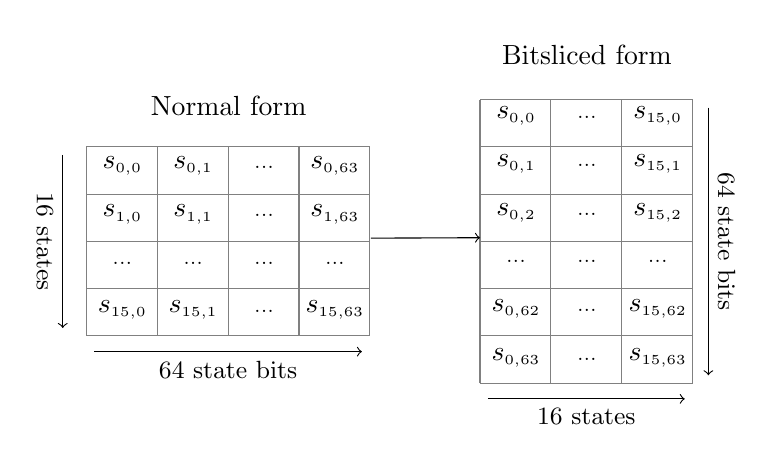
\begin{tikzpicture}
[
     block/.style={rectangle, fill=none, text width=7em, text centered, minimum height=2em},
]

\draw[->] (0.1,-.2) -- (3.5,-.2) node[below,midway] {\small 64 state bits};
\draw[->] (-0.3,2.3) -- (-.3,.1) node[below,midway,sloped] {\small 16 states};
\begin{scope}
\draw[xstep=0.9cm,ystep=0.6,color=gray] (0,0) grid (3.6,2.4);
\matrix[matrix of nodes,
inner sep=0pt,
anchor=south west,
nodes={inner sep=0pt,text width=.9cm,align=center,minimum height=.6cm}
](m1){
$s_{\scriptscriptstyle 0,0}$ & $s_{\scriptscriptstyle 0,1}$ & $\scriptstyle \ldots$ & $s_{\scriptscriptstyle 0,63}$  \\
$s_{\scriptscriptstyle 1,0}$ & $s_{\scriptscriptstyle 1,1}$ & $\scriptstyle \ldots$ & $s_{\scriptscriptstyle 1,63}$  \\
$\scriptstyle \ldots$  & $\scriptstyle \ldots$&$\scriptstyle \ldots$ &$\scriptstyle \ldots$  \\
$s_{\scriptscriptstyle 15,0}$ & $s_{\scriptscriptstyle 15,1}$ & $\scriptstyle \ldots$ & $s_{\scriptscriptstyle 15,63}$  \\
};
 \end{scope}

\node [block,above=.1cm of m1] (text1) {Normal form};

 \begin{scope}[xshift=5cm]
 \draw[->] (0.1,-.8) -- (2.6,-.8) node[below,midway] {\small 16 states};
 \draw[->] (2.9,2.9) -- (2.9,-0.5) node[above,midway,sloped] {\small 64 state bits};
\draw[xstep=0.9cm,ystep=0.6,color=gray] (0,-0.6) grid (2.7,3);
\matrix[matrix of nodes,
inner sep=0pt,
anchor=south west,
nodes={inner sep=0pt,text width=.9cm,align=center,minimum height=.6cm}
] at (0,-0.6)(m2){
$s_{\scriptscriptstyle 0,0}$ &  $\scriptstyle \ldots$ & $s_{\scriptscriptstyle 15,0}$  \\
$s_{\scriptscriptstyle 0,1}$ &  $\scriptstyle \ldots$ & $s_{\scriptscriptstyle 15,1}$  \\
$s_{\scriptscriptstyle 0,2}$ &  $\scriptstyle \ldots$ & $s_{\scriptscriptstyle 15,2}$  \\
$\scriptstyle \ldots$  & $\scriptstyle \ldots$ &$\scriptstyle \ldots$  \\
$s_{\scriptscriptstyle 0,62}$ &  $\scriptstyle \ldots$ & $s_{\scriptscriptstyle 15,62}$  \\
$s_{\scriptscriptstyle 0,63}$ &  $\scriptstyle \ldots$ & $s_{\scriptscriptstyle 15,63}$  \\
};
 \end{scope}
 
 \node [block,above=.1cm of m2] (text1) {Bitsliced form};

\draw[->] (m1) -- (m2);

\end{tikzpicture}
\end{adjustbox}
		\caption{16~cipher states (each 64~bit) in normal form (left) and bitsliced form (on a 16-bit processor, right).}
		\label{fig:symmetric_crypto:bitslicing}
\end{figure} 

Note that storing each entry of $s'$ as one byte is a choice made here for illustrative purposes. Usually, one would select the register size of a processor (i.e., 16~bit for the MSP430, 32~bit for an embedded ARM core such as in the RP2040, 64~bit for a modern \ac{CPU}) to be able to most efficiently make use of the processor's hardware. Of course, this implies that even more cipher instances are computed in parallel (16 for the example of the MSP430, 32 for the RP2040, 64 for a \ac{PC} \ac{CPU}).

\emph{Note:} One actually does not have to explicitly transform the round keys into bitsliced form. Instead, if the same key (and hence the same round keys) are used for all bitsliced blocks, we can make use of the fact that each element (bit) \verb+i+ in the bitsliced \verb+roundkey_exp[i]+ can only either be all 0 (if bit \verb+i+ of the round key is 0) or all 1 (if bit \verb+i+ of the round key is 0). 
%
Hence, the key addition can be rewritten as (pseudocode):
\begin{lstlisting}
for(uint8_t i = 0; i < 64; i++)
{
   if(bit i of roundkey == 1) {
      state[i] = state[i] ^ 0xFFFF...FF;
   }
}
\end{lstlisting}

However, this way causes the runtime of the implementation to be key-dependent, which is generally undesirable. Using the fact that -1 = \verb+0xFFFF...FF+ and that -0 = \verb+0x0000...00+, we can however rewrite this as:
\begin{lstlisting}
for(uint8_t i = 0; i < 64; i++)
{
   // Assume: x is either 1 or 0
   b = get bit i of roundkey;
   state[i] = state[i] ^ -b;
}
\end{lstlisting}

\paragraph{Time and Memory Complexity}
For bit-oriented ciphers like PRESENT or \ac{DES}, bitslicing usually gives a significant performance increase due to the amount of operations saved for the permutations. The key addition layer is similar in performance for normal and bitsliced implementations, while the \ac{SBOX} layer is usually more costly when implemented in bitsliced form. The overhead of the \ac{SBOX} layer depends on the number of required Boolean operations to implement the \ac{SBOX}---hence, finding a representation with as little Boolean operations as possible is crucial for bitsliced implementations with best performance.
%
Besides, the operations to bring the input states into bitsliced form add computational complexity. Hence, it is normally desirable to stay in bitsliced form---and not to ``switch'' between the forms, e.g., to implement an \ac{SBOX} as a \ac{LUT}, converting the input to normal representation and back to bitsliced form afterwards. 
%
In terms of memory, bitslicing generates an overhead since multiple cipher states are stored at the same time. Moreover, the computation of the \ac{SBOX} usually requires (some) temporary registers to buffer the input bits. The code size may increase as well, especially if the \ac{SBOX} requires many Boolean operations.
Overall, bitslicing is highly useful in scenarios where a large amount of data has to be encrypted with a bit-oriented cipher. In contrast, for byte-oriented ciphers like the \ac{AES} (with larger \ac{SBOX}), a table-based implementation will likely give better performance than bitslicing, though bitslicing can offer competitive performance and other advantages such as constant execution time (see \Cref{sec:impl_attacks:sca} for why this is often needed)~\cite{Schwabe17}.

\subsection{The \acl{ANF}}
\label{chap:symmetric_crypto:anf}
This section is supplementary material to the bitslicing section. We will look at one representation of Boolean functions, the \acl{ANF}, including an efficient algorithm to compute the \ac{ANF} from a truth table for a given Boolean function. In this section, we consider a $n$-to-$1$ Boolean function:
$$
y = f\left(x_0,\,x_1,\,\ldots,\, x_{n-1}\right)\ \textrm{where}\ \left(x_0,\,x_1,\,\ldots,\,x_{n-1}\right) \in \binfield{n}\ \textrm{and}\ y \in \binfield{}
$$
The \ac{ANF} is a form to express any such function as the \verb+XOR+ sum of \verb+AND+ combinations of $x_0,\,x_1,\, \ldots$. As an example, for $n = 4$, a function in \ac{ANF} would be:
$$
f\left(x_0,\,x_1,\,x_2,\,x_3\right) = x_0 + x_1 + x_2 \cdot x_3 + x_0 \cdot x_1 \cdot x_3 + x_0 \cdot x_1 \cdot x_2 \cdot x_3
$$
Note that \ac{ANF} is written over binary variables in $\binfield{2}$ (which is equivalent to computing $\mod 2$), hence, $+$ represents \verb+XOR+ and $\cdot$ \verb+AND+. In general, the \ac{ANF} can be expressed as:
$$
f\left(x_0,\,x_1,\,\ldots,\, x_{n-1}\right) = \sum_{u \in \binfield{n}}{\left(\lambda_u \prod_{i = 0}^{n-1}{x_i^{u_i}} \right)} 
$$
with in total $2^n$ coefficients $\lambda_u \in \binfield{}$ (for $u = \left(00\ldots00\right),\,\left(00\ldots01\right),\,\ldots,\,\left(11\ldots11\right)$). Note that there is no ``information loss'' or ``compression'' in the \ac{ANF}---both the truth table and the \ac{ANF} can be described with a bit string of length $2^n$.
%
The \ac{ANF} of any Boolean function can be computed using an \ac{FFT}-like algorithm. The main steps are:

\begin{enumerate}[itemsep=-1pt]
	\item Write the truth table for the function $y = f\left(x_0,\,x_1,\,\ldots,\, x_{n-1}\right)$;
	\item Apply the ``butterfly'' $n$ times, with spacing $\sigma = 2^0 = 1,\,2^1,\,2^2,\,\ldots,\,2^{n-1}$;
	\item The resulting table contains the coefficients $\lambda_u$, where $u = \left(x_0,\,x_1,\,\ldots,\, x_{n-1}\right)$.
\end{enumerate}

whereas the butterfly (for two inputs $a$, $b$, spaced by $\sigma$) is defined as follows:

\begin{figure}[h!tb]
		\center
		\usetikzlibrary{matrix}
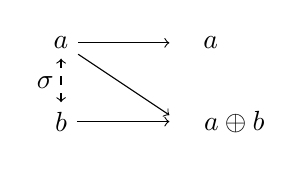
\begin{tikzpicture}
\node (a) at (0,0) {$a$};
\node (b) at (0,-1) {$b$};

\node (a2) at (1.5,0) {};
\node (ab) at (1.5,-1) {$$};

\node at (1.9,0) {$a$};
\node at (2.2,-1) {$a \oplus b$};

\node at (-0.2, -0.5) {$\sigma$};

\draw[->] (a)--(a2);
\draw[->] (a)--(ab);
\draw[->] (b)--(ab);

\draw[<->, dashed] (a)--(b);

\end{tikzpicture}
		\caption{Butterfly for computing \ac{ANF}.}
		\label{fig:symmetric_crypto:butterfly}
\end{figure} 

\paragraph{Example}
The method is best illustrated by an example. Given the following function ($n = 3$):

\begin{figure}[h!tb]
		\center
		\usetikzlibrary{matrix}
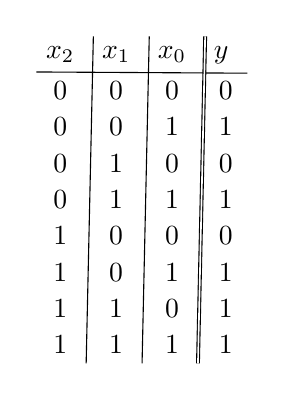
\begin{tikzpicture}
\matrix(dict)[matrix of nodes,%below=of game,
        nodes={align=center},
        %row 1/.style={anchor=south},
        %column 1/.style={nodes={text width=2cm,align=center}}
    ]{
        $x_2$ & $x_1$ & $x_0$ & $y$ \\
	 0 & 0 & 0 &  0\\
	 0 & 0 & 1 &  1\\
	 0 & 1 & 0 &  0\\
	 0 & 1 & 1 &  1\\
	 1 & 0 & 0 &  0\\
	 1 & 0 & 1 &  1\\
	 1 & 1 & 0 &  1\\
	 1 & 1 & 1 &  1\\
    };
    \draw(dict-1-1.south west)--(dict-1-4.south east);
    \draw(dict-1-1.north east)--(dict-9-1.south east);
    \draw(dict-1-2.north east)--(dict-9-2.south east);
    \draw[double](dict-1-3.north east)--(dict-9-3.south east);
\end{tikzpicture}
		\caption{Truth table of example function $y = f\left(x_0,\,x_1, x_2\right)$.}
		\label{fig:symmetric_crypto:anf_tt}
\end{figure} 

The \ac{ANF} is computed as in the following Table~\ref{fig:symmetric_crypto:anf_tt_comp}:

After the final step with spacing $\sigma = 2^2 = 4$, one reads the coefficients that are set to $1$, in this case these are the coefficients for input $001$, $110$, $111$. This means that $\lambda_{001} = \lambda_{110} = \lambda_{111} = 1$, while the remaining $\lambda_u$ are $0$. Hence, we have the \ac{ANF}:

$$
y = f\left(x_0,\,x_1, x_2\right) = x_0 + x_2 \cdot x_1 + x_2 \cdot x_1 \cdot x_0
$$

Note that if $\lambda_{000} = 1$, we would have the term $x_0^0 \cdot x_1^0 \cdot x_2^0 = 1$ in the \ac{ANF}, i.e., the result is inverted ($+1$ is \verb+XOR+ with $1$ or in other words inversion).  

\begin{figure}[h!tb]
		\center
		\usetikzlibrary{matrix}
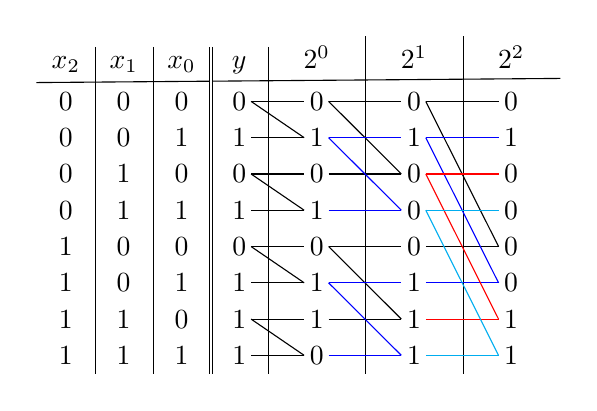
\begin{tikzpicture}

\newcommand{\btf}[5][]
{
  % this needed to be modified somehow...
  \draw[#1] ($(#2) + (0.15,0)$)--($(#3) - (0.16,0)$);
  \draw[#1] ($(#4) + (0.15,0)$)--($(#5) - (0.16,0)$);
  \draw[#1] ($(#2) + (0.15,0)$)--($(#5) - (0.16,0)$);
}

\matrix(dict)[matrix of nodes,%below=of game,
        nodes={align=center,text width=.5cm},
        %row 1/.style={anchor=south},
        column 5/.style={nodes={text width=1cm}},
        column 6/.style={nodes={text width=1cm}},
        column 7/.style={nodes={text width=1cm}}
    ]{
        $x_2$ & $x_1$ & $x_0$ & $y$ & $2^0$ & $2^1$ & $2^2$\\
	 0 & 0 & 0 &  0 & 0 & 0 & 0\\
	 0 & 0 & 1 &  1 & 1 & 1 & 1\\
	 0 & 1 & 0 &  0 & 0 & 0 & 0\\
	 0 & 1 & 1 &  1 & 1 & 0 & 0\\
	 1 & 0 & 0 &  0 & 0 & 0 & 0\\
	 1 & 0 & 1 &  1 & 1 & 1 & 0\\
	 1 & 1 & 0 &  1 & 1 & 1 & 1\\
	 1 & 1 & 1 &  1 & 0 & 1 & 1\\
    };
    \draw(dict-1-1.south west)--(dict-1-7.south east);
    \draw(dict-1-1.north east)--(dict-9-1.south east);
    \draw(dict-1-2.north east)--(dict-9-2.south east);
    \draw[double](dict-1-3.north east)--(dict-9-3.south east);
    \draw[](dict-1-4.north east)--(dict-9-4.south east);
    \draw[](dict-1-5.north east)--(dict-9-5.south east);
    \draw[](dict-1-6.north east)--(dict-9-6.south east);
    
    % First round
    \btf{dict-2-4}{dict-2-5}{dict-3-4}{dict-3-5};
    \btf{dict-4-4}{dict-4-5}{dict-5-4}{dict-5-5};
    \btf{dict-6-4}{dict-6-5}{dict-7-4}{dict-7-5};
    \btf{dict-8-4}{dict-8-5}{dict-9-4}{dict-9-5};
    
    % Second round
    \btf{dict-2-5}{dict-2-6}{dict-4-5}{dict-4-6};
    \btf[color=blue]{dict-3-5}{dict-3-6}{dict-5-5}{dict-5-6};
    \btf{dict-6-5}{dict-6-6}{dict-8-5}{dict-8-6};
    \btf[color=blue]{dict-7-5}{dict-7-6}{dict-9-5}{dict-9-6};
    
       % Third round
    \btf{dict-2-6}{dict-2-7}{dict-6-6}{dict-6-7};
   \btf[color=blue]{dict-3-6}{dict-3-7}{dict-7-6}{dict-7-7};
   \btf[color=red]{dict-4-6}{dict-4-7}{dict-8-6}{dict-8-7};
   \btf[color=cyan]{dict-5-6}{dict-5-7}{dict-9-6}{dict-9-7};
    
 %   \btf{dict-4-4}{dict-4-5}{dict-5-4}{dict-5-5};
 %   \btf{dict-2-4}{dict-2-5}{dict-3-4}{dict-3-5};
 %   \btf{dict-2-4}{dict-2-5}{dict-3-4}{dict-3-5};
    
    
    
\end{tikzpicture}
		\caption{Computation of \ac{ANF} of example function $y = f\left(x_0,\,x_1, x_2\right)$.}
		\label{fig:symmetric_crypto:anf_tt_comp}
\end{figure} 





%---------------------------------------------------------------------




